\documentclass[conference]{IEEEtran}
\usepackage{amsmath,amssymb}
\usepackage{graphicx}
\usepackage{booktabs}
\usepackage{array}
\usepackage{url}
\usepackage{xurl}
\usepackage[colorlinks=true,linkcolor=black,citecolor=black,urlcolor=blue]{hyperref}
\usepackage{listings}
\usepackage{tikz}
\usetikzlibrary{arrows.meta,positioning,fit,calc}
\usepackage{balance}

\lstset{
  language=Python,
  basicstyle=\ttfamily\scriptsize,
  keywordstyle=\color{blue!60!black},
  breaklines=true,
  frame=single,
  rulecolor=\color{gray!40},
  columns=fullflexible,
  showstringspaces=false
}

\begin{document}

\title{Autonomous Repository Engineer:\\
A Verified Tool-Using Coding Agent with Deterministic Governance}

\author{\IEEEauthorblockN{Vaibhav Mahore}
\IEEEauthorblockA{\textit{Department of Mathematics and Computing}\\
\textit{Indian Institute of Science, Bangalore, India}\\
mvaibhav@iisc.ac.in}}

\maketitle

\begin{abstract}
LLM-based coding agents typically fail in one of three ways: they parse
free-text tool calls until the model produces a malformed one, they hand the
model a shell, or they accept the model's claim that a task is complete.
This paper presents the Autonomous Repository Engineer, a coding-agent
runtime organized around an explicit governance principle: the model
proposes actions, the runtime validates and executes them, the repository
state provides observations, and completion is accepted only on verification
evidence. A deterministic finite state machine (INIT, ANALYZE\_REPO, PLAN,
ACT, OBSERVE, REPLAN, VERIFY, COMPLETE, FAILED, with a HUMAN\_REVIEW
branch) wraps a pluggable planner; seven tools are invoked exclusively
through schema-validated calls subject to a workspace path jail,
AUTO/ASK/DENY permission policies, and a test-command allowlist; and the
VERIFY state re-runs the test suite, accepting completion only on an
\texttt{exit=0} observation. On a four-task benchmark (bug fix, failing
test, missing test, constrained refactor) run in isolated workspace copies
with a deterministic scripted planner, the agent completes 4/4 tasks with
zero failed tool calls. With a live Gemini 2.5 Flash planner proposing JSON
tool calls through the same validated runtime, the agent completes 2/2
tasks, absorbing two provider rate-limit errors mid-run through a bounded
planner-error recovery path. Every run emits a serializable execution trace.
The benchmarks are deliberately small: they demonstrate the governance
machinery and the live integration, not general coding capability, and the
paper preserves the project's scope limits (scripted planner as a fixture,
no OS-level sandboxing, no transactional rollback) explicitly.
\end{abstract}

\begin{IEEEkeywords}
LLM agents, tool use, software engineering automation, sandboxing, verification, state machines
\end{IEEEkeywords}

\section{Introduction}
Repository-level coding agents promise automation of small engineering
tasks: fixing a bug, repairing a failing test, adding coverage, or
refactoring an interface. Deploying an LLM for these tasks exposes three
recurring failure modes. First, \emph{interface fragility}: models
hallucinate tool names, omit required arguments, or misuse types, and a
runtime that parses free text crashes with them. Second, \emph{excessive
authority}: giving a model a shell prompt couples its correctness to host
security. Third, \emph{unverified completion}: a model can assert success
regardless of repository state, and a pipeline that trusts the assertion
automates nothing reliable.

Prior agent designs address these partially. ReAct-style loops
\cite{yao2023react} interleave reasoning and acting but leave execution
policy implicit. Toolformer \cite{schick2023toolformer} learns tool
invocation but targets self-supervised API use rather than repository
mutation under governance. SWE-bench \cite{jimenez2024swebench} establishes
that repository-level fixing is hard at scale, but its harness measures
capability, not the safety architecture around a model.

The Autonomous Repository Engineer treats governance as the primary design
object. Its principle, enforced in code rather than prompt text, is:

\begin{quote}
\emph{The model proposes actions. The runtime validates and executes them.
The repository state provides observations. Completion is accepted only
after verification evidence.}
\end{quote}

The contributions are: (1) a planner/executor split in which every planner
output flows through one validation pipeline regardless of whether the
planner is a deterministic script or a live LLM (Section~III); (2) a
tool layer with typed schemas, permission classes and policies, a workspace
path jail, and a command allowlist (Section~IV); (3) a state-machine runtime
with step, replan, and planner-error budgets and test-gated completion
(Section~V); (4) a reproducible four-task benchmark and a live Gemini run
recorded separately (Section~VI); and (5) an explicit account of residual
risks (Section~VII).

\section{System Overview}
Fig.~\ref{fig:arch} shows the division of authority. The planner (scripted
recipes, a recorded replay, or an LLM over an OpenAI-compatible endpoint)
emits one structured proposal per turn: a tool name and an argument object,
or a \texttt{done} declaration. The runtime alone decides what happens:
known tool, schema-conformant arguments, permission policy, and workspace
containment are all checked before any effect; rejected proposals become
observations returned to the planner rather than exceptions. The state
machine advances through ANALYZE\_REPO, PLAN, ACT, OBSERVE, and either back
to PLAN, to REPLAN (on test failure), or to VERIFY, which re-runs the test
suite through the same allowlisted tool; COMPLETE is reachable only from
VERIFY, and only on an \texttt{exit=0} observation. Step, replan, and
consecutive-planner-error budgets bound every run; exhausted budgets end in
FAILED with a full trace.

\begin{figure*}[t]
\centering
\resizebox{\textwidth}{!}{
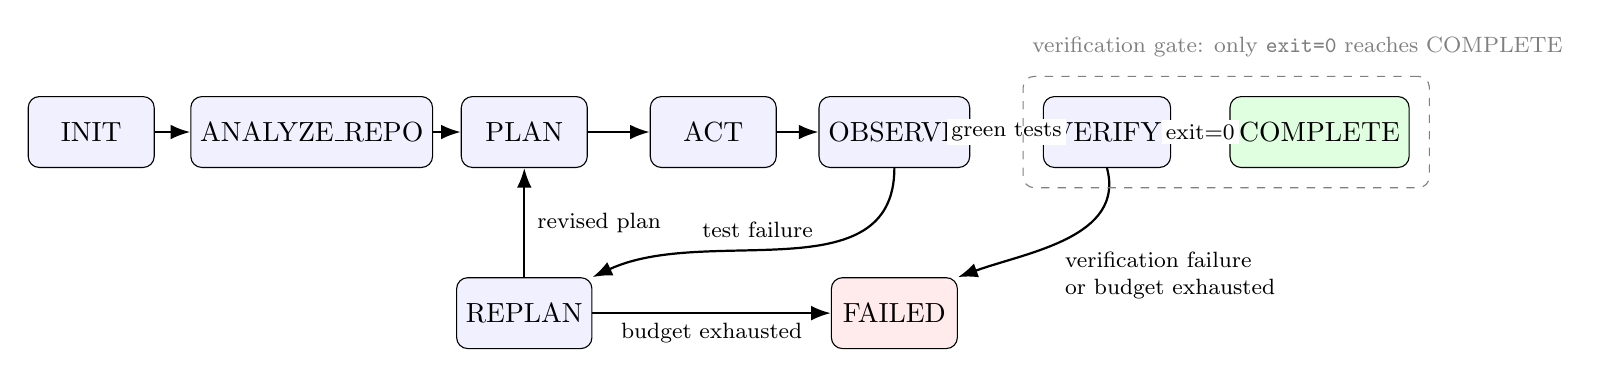
\begin{tikzpicture}[x=1cm,y=1cm,
  st/.style={draw, rounded corners, fill=blue!6, minimum height=9mm,
             minimum width=16mm, align=center},
  ter/.style={st, fill=green!12},
  bad/.style={st, fill=red!8},
  arr/.style={-{Latex[length=2.5mm]}, thick},
  lab/.style={font=\footnotesize, fill=white, inner sep=1.5pt}]
% ---- row 1: main path ----
\node[st] (init)    at (0.0, 0)    {INIT};
\node[st] (ana)     at (2.8, 0)    {ANALYZE\_REPO};
\node[st] (plan)    at (5.5, 0)    {PLAN};
\node[st] (act)     at (7.9, 0)    {ACT};
\node[st] (obs)     at (10.2, 0)   {OBSERVE};
\node[st] (verify)  at (12.9, 0)   {VERIFY};
\node[ter] (done)   at (15.6, 0)   {COMPLETE};
% ---- row 2: failure handling ----
\node[st] (replan)  at (5.5, -2.3) {REPLAN};
\node[bad] (failed) at (10.2, -2.3) {FAILED};
% ---- main-path arrows ----
\draw[arr] (init)   -- (ana);
\draw[arr] (ana)    -- (plan);
\draw[arr] (plan)   -- (act);
\draw[arr] (act)    -- (obs);
\draw[arr] (obs)    -- node[lab]{green tests} (verify);
\draw[arr] (verify) -- node[lab]{exit=0} (done);
% ---- failure branch: OBSERVE -> REPLAN -> PLAN ----
\draw[arr] (obs.south) to[out=-90,in=25]
  node[lab, pos=0.4, above left=0.5mm]{test failure} (replan.north east);
\draw[arr] (replan.north) -- node[lab, right=1mm]{revised plan} (plan.south);
% ---- failure exits to FAILED ----
\draw[arr] (replan) -- node[lab, below=0.6mm]{budget exhausted} (failed);
\draw[arr] (verify.south) to[out=-75,in=20]
  node[lab, pos=0.55, below right=0.4mm and 0.6mm, align=left]
  {verification failure\\or budget exhausted} (failed.north east);
% ---- invariant: the verification gate ----
\node[draw=gray, dashed, rounded corners, inner sep=2.5mm,
      fit=(verify)(done)] (gate) {};
\node[font=\footnotesize, gray, above=1.2mm of gate.north west,
      anchor=south west]
      {verification gate: only \texttt{exit=0} reaches COMPLETE};
\end{tikzpicture}}
\caption{Runtime state machine of the Autonomous Repository Engineer.
Planner proposals pass through the validated execution pipeline before any
state advances; test failures trigger bounded replanning (REPLAN returns to
PLAN; exhausted budgets end in FAILED from either REPLAN or VERIFY); and
completion is reachable only from VERIFY, after an \texttt{exit=0}
observation from the allowlisted test tool. The HUMAN\_REVIEW branch is
omitted for space.}
\label{fig:arch}
\end{figure*}

The machine is strict: transitions not present in the adjacency table raise
errors rather than drifting, PLAN-to-PLAN self-loops are collapsed, and the
agent state (plan, actions, observations, test results, budgets, hypothesis,
changed files) is serializable to JSON, so every run leaves a reviewable
artifact.

\section{Tool Layer}
Seven tools cover the tasks the agent may perform: \texttt{list\_tree},
\texttt{search}, \texttt{read\_file}, \texttt{apply\_edit},
\texttt{write\_file}, \texttt{git\_diff}, and \texttt{run\_tests}. Each is
declared as a specification containing its name, description, permission
class, required and optional typed arguments, and implementation; the
registry rejects unknown tools, missing or mistyped arguments, and unknown
argument keys before anything executes. Three policies are worth describing
because they carry most of the safety argument.

\textbf{Workspace path jail.} Every path argument is resolved against the
workspace root and must remain within it:
\begin{lstlisting}
def jailed_path(self, raw: str) -> Path:
    candidate = Path(raw)
    resolved = (candidate.resolve() if candidate.is_absolute()
                else (self.workspace / candidate).resolve())
    if resolved != self.workspace and
       self.workspace not in resolved.parents:
        raise PermissionError("path escape rejected")
    return resolved
\end{lstlisting}
Because \texttt{resolve()} collapses \texttt{..} segments and resolves
symlinks, traversal attempts such as \texttt{../outside.txt} or absolute
paths outside the workspace resolve to locations that fail the ancestor
check. Unit tests exercise \texttt{..}, absolute, and drive-letter escapes.

\textbf{Unambiguous mutation.} \texttt{apply\_edit} replaces exactly one
occurrence of an exact string: zero matches and multiple matches are both
errors, so a planner that misread a file cannot silently clobber it.
\texttt{write\_file} refuses to overwrite existing files, forcing new
content through an explicit creation step. Both restrictions convert
``the model wrote something unexpected'' into a structured, recorded
rejection.

\textbf{Execution allowlist.} \texttt{run\_tests} is the only execution
tool. It accepts only command prefixes from an allowlist (by default
\texttt{python -m pytest} and \texttt{python -m unittest}), executes
without a shell, with a subprocess timeout, and with output captured and
capped. A proposal such as \texttt{curl~...~|~sh} is rejected by the
prefix check before any process exists.

Permission classes (READ\_ONLY, MUTATING, EXECUTION) map to policies
(AUTO, ASK, DENY). ASK requires an approval callback and denies by default
when none is configured (fail closed), which makes headless runs safe by
construction. Rejections are first-class observations: they are recorded in
the trace and returned to the planner as history, so a malformed proposal
costs a turn, not a crash.

\section{Runtime and Verification}
The runtime loop maintains three budgets: a step budget (40), a replan
budget (4), and a consecutive-planner-error budget (3), so the worst case
of a confused planner is bounded in steps, cost, and damage. A failed test
run transitions OBSERVE to REPLAN; exhausted replans or planner errors end
the run in FAILED. On planner proposal of \texttt{done}, the runtime
transitions to VERIFY and re-executes the suite itself; the planner's claim
is never consulted. Files changed by accepted edits are tracked in the
agent state, and the full state serializes to a JSON trace for offline
audit.

The planner interface has three implementations with distinct, stated
roles. \texttt{ScriptedPlanner} replays deterministic per-task recipes: it
is a test fixture that exercises the runtime machinery at zero cost and
full reproducibility, and it is not presented as intelligence.
\texttt{LLMPlanner} packages the task description, the tool catalog, and
the last ten history entries (with truncated outputs) into a prompt and
parses a JSON reply; proposals then pass through the identical validation
pipeline. \texttt{RecordedPlanner} replays captured actions for tests
without network access.

\section{Evaluation}

\subsection{Deterministic Benchmark}
Four self-contained task repositories are copied into fresh workspaces per
run (isolation), and the agent runs with the scripted planner
(Table~\ref{tab:det}). All four tasks complete with zero failed tool calls;
task 02's first test run fails by construction (the suite detects the
bug), producing the single replan; total wall time is under five seconds.
The benchmark measures the runtime machinery (validation, jail, policies,
state transitions, verification) and nothing about model capability.

\begin{table}[t]
\centering
\caption{Deterministic benchmark (scripted planner, isolated workspace
copies).}
\label{tab:det}
\small
\begin{tabular}{@{}lrrrr@{}}
\toprule
Task & Success & Steps & Replans & Wall (s) \\
\midrule
fix off-by-one loop & yes & 5 & 0 & 0.99 \\
repair failing test & yes & 5 & 1 & 1.46 \\
add missing test & yes & 5 & 0 & 0.96 \\
constrained refactor & yes & 7 & 0 & 0.95 \\
\midrule
Total & 4/4 & 22 & 1 & 4.36 \\
\bottomrule
\end{tabular}
\end{table}

\subsection{Live Gemini Benchmark}
With \texttt{LLMPlanner} backed by Gemini 2.5 Flash (temperature 0) through
an OpenAI-compatible endpoint, the agent was run on two of the four tasks
(Table~\ref{tab:live}). Both complete with zero failed tool calls. On the
open-ended task (adding a test file) the model wrote its own test cases
rather than reproducing the scripted recipe. The run also exercised the
error-recovery path: two HTTP 429 provider errors occurred mid-task and
were absorbed as recoverable planner errors by the provider's backoff and
the runtime's budget accounting, with the runs ending in verified
completion.

\begin{table}[t]
\centering
\caption{Live planner run (Gemini 2.5 Flash). Per-task LLM counters in the
committed JSON are cumulative snapshots because one planner instance was
shared across tasks; true totals are 7 calls, 3{,}887 prompt and 518
completion tokens (the committed summary line of 11 calls double-counts
task 01; both figures are recorded in the repository).}
\label{tab:live}
\small
\begin{tabular}{@{}lrrrr@{}}
\toprule
Task & Success & Steps & LLM calls & Wall (s) \\
\midrule
fix off-by-one loop & yes & 5 & 4 & 10.0 \\
add missing test & yes & 4 & 3 & 49.6 \\
\midrule
Total & 2/2 & 9 & 7 & 59.6 \\
\bottomrule
\end{tabular}
\end{table}

Scope statement: two tasks, one run, one provider. This demonstrates the
integration: a live model proposing actions that survive the governance
pipeline and produce verified completions, and nothing more. It is not a
SWE-bench result, and the deterministic benchmark does not evidence general
coding ability.

\section{Limitations}
(1) The scripted planner is a fixture; without wiring \texttt{LLMPlanner}
to a capable model, the benchmark says nothing about model-driven
competence beyond the two live tasks. (2) Sandboxing is at the application
layer (path jail, allowlist, timeouts); a production deployment would add
OS-level isolation. (3) There is no transactional rollback of edits; the
trace is the review artifact. (4) \texttt{HUMAN\_REVIEW} exists in the
state machine but is never automatically triggered; interactive approval is
wired through the ASK policy only. (5) The tool set is intentionally
minimal; multi-file semantic edits and build systems are out of scope.
(6) File contents returned by tools enter the planner's context, so
prompt-injection resistance ultimately depends on the planner treating
observations as data; the runtime bounds the damage any injection can do.

\section{Conclusion}
The Autonomous Repository Engineer demonstrates that the interesting
engineering problem in coding agents is not the model but the governance
around it: typed tool schemas with unambiguous mutation semantics, a path
jail and allowlists that make dangerous actions structurally unavailable,
budgets that bound every run, and a verification gate that accepts
completion only on test evidence. The deterministic benchmark shows the
machinery working 4/4 with zero failed tool calls at negligible cost; the
live Gemini run shows a real model's proposals surviving the same pipeline
2/2, including recovery from provider failures. Traces make every run
auditable, and the project's limits (fixture planner, application-layer
sandboxing, small benchmark) are part of its published
specification.\footnote{\url{https://github.com/vaibhav3000/repo-engineer}}

\begin{thebibliography}{4}

\bibitem{yao2023react}
S.~Yao, J.~Zhao, D.~Yu, N.~Du, I.~Shafran, K.~Narasimhan, and Y.~Cao,
``ReAct: Synergizing reasoning and acting in language models,'' in
\emph{Int. Conf. on Learning Representations (ICLR)}, 2023,
arXiv:2210.03629.

\bibitem{schick2023toolformer}
T.~Schick, Y.~Dwivedi-Yu, R.~Dessi, R.~Ancilotti, A.~Fan, and
J.~Grave, ``Toolformer: Language models can teach themselves to use
tools,'' 2023, arXiv:2302.04761.

\bibitem{jimenez2024swebench}
C.~E. Jimenez, J.~Yang, A.~Wettig, S.~Yao, K.~Pei, O.~Press, and
K.~Narasimhan, ``SWE-bench: Can language models resolve real-world GitHub
issues?'' in \emph{Int. Conf. on Learning Representations (ICLR)}, 2024,
arXiv:2310.06770.

\bibitem{wang2024codeact}
X.~Wang, Y.~Chen, L.~Yuan, Y.~Zhang, Y.~Li, H.~Peng, and H.~Ji,
``Executable code actions elicit better LLM agents,'' in \emph{Proc. Int.
Conf. on Machine Learning (ICML)}, 2024, arXiv:2402.01030.

\end{thebibliography}

\end{document}
